\chapter{Detecção de clones}\label{chap clonedt}
\minitoc

Os primeiros passos para a implementação da detecção de clones na aplicação já tinha sido dados anteriormente, quando se começou por escrever um script em Perl para o efeito. O script já foi descrito em secções anteriores, no entanto apenas agora foi integrado na aplicação. Como nesse processo sofreu algumas alterações, vamos voltar a explicá-lo ao pormenor.

\section{Modo de utilização}
O script tem como finalidade comparar dois ficheiros, e verificar se foram detectadas possíveis cópias, entre os dois. Desta forma o script ao ser chamado, recebe dois ficheiros como input:
\begin{itemize}
\item perl cloneDt -file \textit{path1} -comp \textit{path2}
\end{itemize}
sendo que \textit{path1} representa o path do ficheiro que se está a testar e \textit{path2} representa o path do ficheiro com o qual se pretende comparar.\\

\section{Processamento do código}
Para que seja possível detectar possíveis clones, mesmo depois de o grupo que está a submeter a cópia ter alterado por exemplo o nome a algumas variáveis ou trocado algumas funções de ordem, é necessário fazer um processamento do código fonte, generalizando ou eliminado alguns dos componentes de um programa.\\
Para tal, o script efectua uma série de procedimentos que irão ser descritos de seguida:
\begin{itemize}
\item começa por executar o comando \textit{ctags -x path1}, de forma a obter a linha em que começa cada função do ficheiro C em questão;
\item guarda num array o código desse ficheiro, dividindo cada função por uma posição diferente do array;
\item elimina comentários uni e multi-linha, da linguagem C;
\item substituí todas as varáveis e tipos por \textit{var} ;
\item substituí todos os números por \textit{1};
\item elimina todos os espaços;
\item de seguida efectua os mesmos passos para o segundo ficheiro;
\item compara cada elemento do primeiro array gerado, com os elementos do segundo;
\end{itemize}

\section{Output	}
O script no fim de comparar os dois arrays, no caso de ter detectado uma possível cópia em pelo menos uma função, imprime a percentagem de funções nas quais foram detectadas cópias.

\section{Integração com a aplicação}
Sempre que uma tentativa é submetida no sistema, o script é executado, comparando os ficheiros C que acabou de submeter com os ficheiros C das tentativas mais recentes, referentes ao mesmo enunciado, dos restantes grupos.\\
No caso de se detectar um possível clone, é inserida uma nova entrada na base de dados, com a informação referente a este evento.\\
A qualquer momento o administrador pode consultar esta lista de warnings, e se achar que foi um falso positivo, pode eliminar a entrada da lista. Ainda na listagem pode aceder ao código dos ficheiros em que se detetou o possível clone.


\begin{figure}[htbp]
\begin{center}
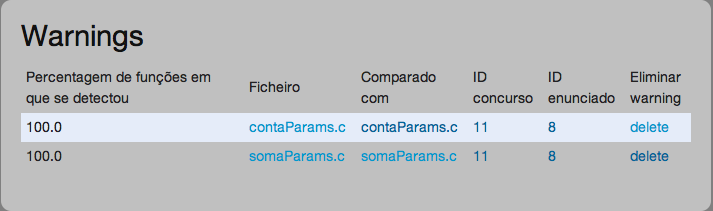
\includegraphics[width=0.9\textwidth]{Images/clone_warning_index}
\caption{Listagem dos warnings}\label{fig clone_index}
\end{center}
\end{figure}